\chapter{Liquid Xenon Dark Matter Detectors}\label{chap:2}
The LUX detector and its upcoming successor, the LUX-ZEPLIN (LZ) detector, have been on the cutting edge of direct detection limits since 2013. These are examples of two-phase xenon time-projection chambers (TPC's). The strongest current limits on WIMP mass and scattering cross-section are placed by measurements using this specific type of detector. In this chapter we will examine what makes xenon as a detector medium so attractive. We will present on the design and operation of LUX, and will develop tools needed to model interactions within the detector.

\section{Xenon as a Detector Medium}
\subsection{Noble Gasses}
Noble gasses are chemically inert, which gives them several properties that make them exciting candidates as WIMP detection media. An interaction of an energetic particle with a target atom will transfer some or all of the particle's energy to the target material. This transferred energy is divided into three channels: scintillation light, free charge, and heat. In a noble gas, the light subsequent to the excitation of an atom will be generated at a wavelength to which the gas is transparent. This scintillation light can therefore be collected and measured.

A noble gas detector will also be sensitive to the charge channel. Free electrons within the medium can be long-lived ($>$1ms), assuming the gas has been purified of more chemically active contaminants. This gives experimenters the chance to extract the free electrons created by an interaction. Since the noble elements are inert, it is also fairly easy to remove problematic impurities by chemical means such as a heated zirconium getter, as used by LUX and LZ.

Typically, detectors that use a noble element as a target have access to one or both of these two channels: charge and light. It is difficult to measure a heat deposit in a liquid or gas-phase detector, but it has been suggested that it may possible to gain access to this channel using a bubble chamber\cite{bubble}. Alternatively, cryogenic solid state experiments are able to measure phonons from interactions. The SuperCDMS experiment, for instance, uses a set of silicon and germanium detectors cooled to 30 mili-Kelvin as its target material\cite{cdms}. Heat-detectors tend to outperform charge and light detectors at low-WIMP masses, because in this regime the charge and light signals start to drop below their respective thresholds.

The relative amount of energy measured in the three channels can be used to help determine whether the interaction of the incident particle with the xenon atom was an electronic recoil (ER) where the particle scattered with an orbital electron, or a nuclear recoil (NR) in which it scattered with the nucleus. This determination allows for strong background rejection, since most low-energy backgrounds are $\beta$'s and $\gamma$'s, which only scatter electronically, while WIMP's, which interact via the weak force, will scatter off of the nucleus. Access to the heat channel would provide greatly improved discrimination between ER events, in which nearly all of the energy is initially divided between charge and light, and NR events, in which a comparatively large portion of the energy goes into heat.

The most common noble elements used in WIMP detection experiments are argon and xenon. Neon has also been used in the DEAP/CLEAN collaboration\cite{clean1,clean2}. Guo and McKinsey also propose the use of superfluid helium\cite{he_dm}. The lighter noble gasses, helium and neon, are complementary to experiments that use argon or xenon because they are more sensitive to low-mass WIMPs ($<$ 10 GeV), whose interactions with the heavier elements would be kinematically suppressed.

\subsection{Xenon Density}
Xenon is perhaps the most exciting candidate of the noble gasses, in part because it is the heaviest stable noble element. It has, on average, 131.3 nucleons in its nucleus, and at its triple point, has a liquid density of 2.978 g/cc. This is higher than the density of aluminum. As was shown in section \ref{sec:wimpcrosssection}, the scattering cross section of a WIMP with an atom with $A$ nucleons is proportional to $A^2$, so a larger atom typically means a better sensitivity. 

The high density also has its own benefit, independent of the scattering cross section. Low-energy electronic backgrounds, such as $\gamma'$s and $\beta$'s, will generally be stopped within a centimeter in the liquid xenon. External backgrounds, and those generated on the detector walls will therefore be highly suppressed at the center of the detector. This is referred to as ``self-shielding'', and allows for greatly improved background rejection. A detector that can reconstruct the location at which an event occurred will be able to fiducialize its volume, assigning more weight to an event near the center of the detector than one near the wall. A simple version of this would be to define some subset of the detector as a ``fiducial volume'', and apply a strict cut, rejecting any event that occurs outside of the fiducial region and accepting any event that occurs within it.
\begin{figure}[h!]
\centering
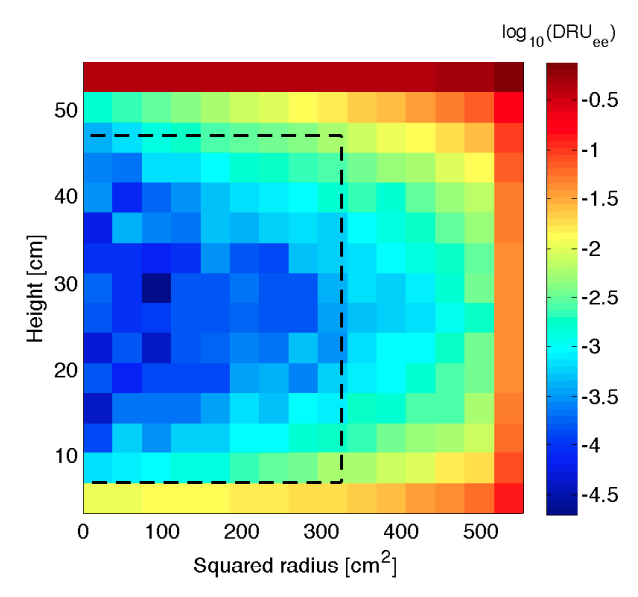
\includegraphics[width=\linewidth]{Figures/lux_fiducial.png}
\caption{Simulated electronic backgrounds in the LUX detector, from 0.9 to 5.3 keV. The black outline shows the 118 kg fiducial which was used to analyze the Run03 data.\cite{lux_fiducial}}
\label{fig:lux_fiducial} 
\end{figure}

\clearpage
\subsection{Radiopurity}
In order for the self-shielding to be effective, the xenon must be free of any dissolved radioactive impurity, and must itself not have any long-lived radioactive isotopes. There are several cosmogenically activated xenon isotopes, but these all have a half life of less than two weeks. They will therefore be suppressed by long-term storage of the xenon underground.

Krypton, for instance, would not be a good candidate for a detector material because it has a relatively large atmospheric abundance of the radioactive isotope $^{85}$Kr, roughly 20 parts per trillion ($^{85}$Kr/$^{nat}$Kr). In fact, for xenon to be used as a WIMP target material, it must first be meticulously cleansed of even trace amounts of krypton. Krypton-85 undergoes a beta-decay with a Q-value of 687 keV and a half life of 10.8 years. It is sourced into the atmosphere by anthropogenic fission to a specific activity of about 1 Bq per cubic meter of air. 

In order to hold the krypton-85 activity below the average expected background rate, the LUX goal was to limit the krypton concentration to less than 5 parts per trillion (grams $^{nat}$Kr per gram Xe). This corresponds to about 700 atoms of $^{85}$Kr per kilogram of xenon, or an activity of about 2$\times \ 10^{-3}$ events/day per kg of xenon per keV. LZ plans to have over 150 times the exposure that LUX had, so in order to keep the number of krypton-85 events constant, it has set a goal of 0.015 parts per trillion\cite{lz_tdr}. 

As mentioned previously, it can be difficult to separate noble gasses from each other. The fact that they are inert means that chemical means are a non-starter. The removal of krypton from xenon is typically done using mass-sorting techniques, such as distillation or mass chromatography. LUX and LZ rely on the latter technique, which has been demonstrated to be effective down to at least 200 ppq (0.2 ppt)\cite{lz_tdr,lux_krremoval}.

Since the required decay rate of $^{85}$Kr is so low, a factor of 10 or even 100 times increase over the concentration limit would not be obvious in the data until weeks or months had passed. It would then take on the order of a year to reprocess the xenon and try again. It is therefore important to have in-situ measurements of the krypton concentration at every step of the construction and operation of a xenon dark matter experiment. Typical mass-spectrometers can only detect concentrations down to about 1 part per million, which is six orders of magnitude too high. LUX and LZ use a technique that was initially developed by Leonard et. al., which augments commercially available mass spectrometers to allow for detection of trace gasses in xenon down to $<$1 ppt\cite{sampling_doug}. In chapter \ref{chap:sampling}, we present methods to improve this technique in order to achieve sensitivities down to the order of 1 ppq. 

There is also an atmospheric component of the radioactive $^{39}$Ar isotope that must be removed from the xenon before it can be used as an effective WIMP detection medium. This isotope has a lower activity in the atmosphere than does $^{85}$Kr. Additionally, because argon is more different in mass from xenon than krypton is, techniques used to detect and remove krypton from xenon will simultaneously and more effectively detect and remove argon.

\section{The LUX Detector}
\subsection{Overview}
LUX and its successor, LZ, are examples of dual-phase, gas/liquid xenon time projection chambers (TPC). TPC's in general can provide a 3D reconstruction of the event position, allowing the internal volume to be fiducialized in order to exploit xenon's self-shielding properties. Specifically, a two phase detector is well suited for WIMP detection, because it produces an amplified charge signal. 

Before it was decommissioned, LUX was located in the Davis cavern at the Sanford Underground Research Facility (SURF) in Lead, South Dakota. It is 4850 feet underground (4300 m w.e.) in order to shield it from cosmic rays. The detector itself was immersed in a large water tank to further shield it from neutrons and gammas. LUX contained about 370 kg of xenon and used a fiducial volume containing about 118 kg as its WIMP target. The remaining xenon acts as a shield from external gammas and betas. The LZ detector will be installed in the same water tank in the Davis cavern, and is slated to have about 20 times the total active xenon mass (7,000 kg) and nearly 50 times the fiducial mass (5,600 kg). The LUX detector has since been removed from its home in the Davis campus and is now on display in the SURF visitor center. 
\begin{figure}[h!]
\centering
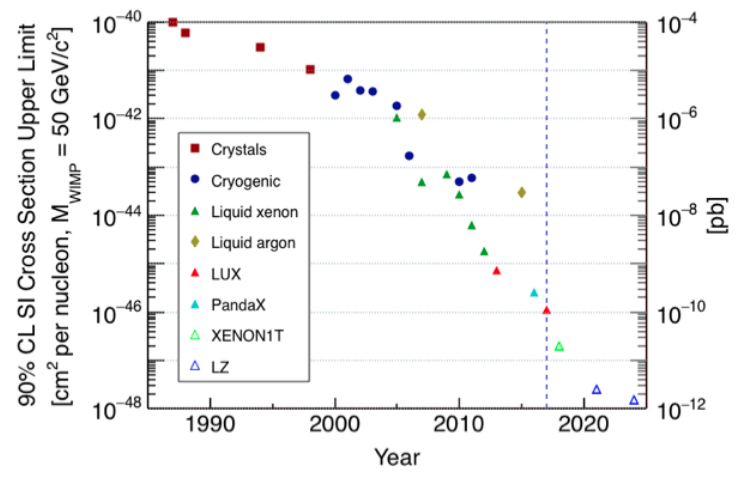
\includegraphics[width=\linewidth]{Figures/limits_trend.png}
\caption{Experimental limits on spin-independent WIMP-nucleon cross section. Figure taken from \cite{lz_tdr}. The open points represent projected limits. The XENON-1T preliminary point is not shown in this plot.}
\label{fig:limits_trend} 
\end{figure}

The LUX full exposure of 3.35 $\times \ 10^4$ kg days yielded the world-leading limit on the spin-independent, WIMP-nucleon scattering cross section. The strongest limit was for a 50 GeV/c$^2$ WIMP, for which cross-sections greater than 1.1 $\times \ 10^{-46}$ cm$^2$ are excluded with 90\% confidence. This result has since been improved on by the XENON-1T experiment, which has set a limit of 7.7 $\times \ 10^{-47}$ cm$^2$ on a 35 GeV/c$^2$ WIMP using a preliminary subset of its full exposure. The full exposure for XENON-1T is expected to improve this limit by about a factor of 5, with an expected limit of about 2 $\times \ 10^{-47}$ cm$^2$ on a 50 GeV/c$^2$ WIMP. The LZ experiment has a projected limit of about another factor of 10 below that.


\subsection{Anatomy of an Event}
An energetic particle that interacts with one of the target xenon atoms in LUX, deposits energy in the form of freed electrons, 178 nm scintillation light, and heat. Two arrays of 61 PMT's at the top and bottom of the detector detect the light emitted from this interaction as primary scintillation ($S1$). All told, LUX contains 122 The Hamamatsu R8778 PMT's, each having an average total quantum efficiency of 30\%. The $S1$ light is directed toward the PMT arrays by Teflon panels which line the interior walls of the detector. When cooled to liquid xenon temperature, Teflon (PTFE) is highly reflective to xenon scintillation light\cite{ptfe_ref}. Combining the collection efficiency with the conversion efficiency of the PMT's, LUX will see about 1 photo-electron for every 11 $S1$ photons emitted from an event site.
\begin{figure}[!h]
\centering
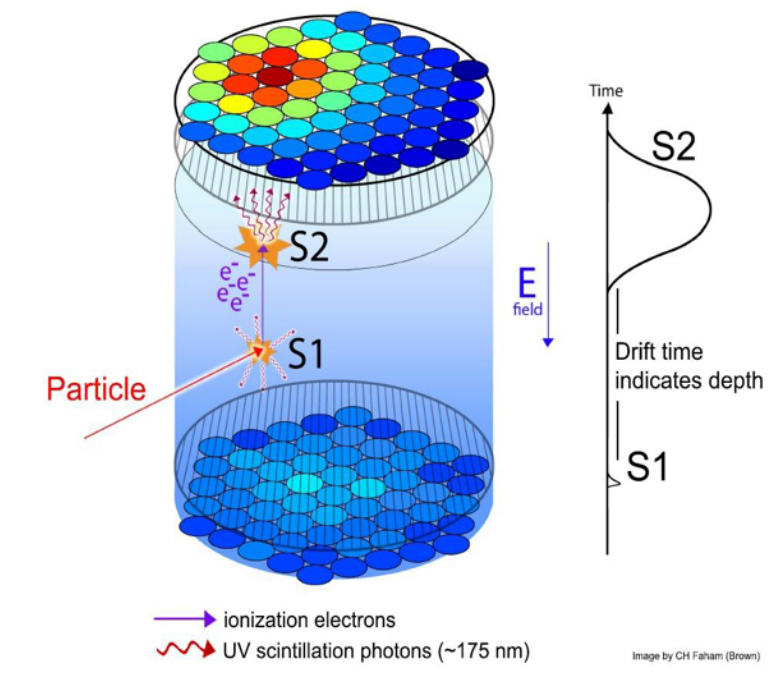
\includegraphics[width=150mm]{Figures/luxevent.png}
\caption{Schematic drawing of an event in the LUX detector. The initial event generates an initial burst of light, which is referred to a primary scintillation or $S1$, along with electron-ion pairs. The electrons are drifted to the liquid surface and extracted, causing a secondary burst of scintillation light, which is called the $S2$ signal. The x-y position of the event can be measured by the location of the $S2$ event, while the depth at which the event occurred is given by the time difference between the $S1$ and $S2$. This time delay is referred to as drift time. Figure taken from \cite{lux2012}.}
\label{fig:lux} 
\end{figure}

The free electrons are separated from the event site through the use of an an electric field, which is referred to as the drift field. They travel through this drift field until they reach the liquid/gas interface, where they are extracted with an efficiency of about 70\%. The voltages around the liquid/gas interface are arranged such that the electric field is about 5 kV/cm just below the surface and 10 kV/cm in the gas. These two field regions are referred to as the extraction field and electro-luminescence field. Once extracted from the liquid, an electron is accelerated through the electro-luminescence field until it gains enough momentum to excite a gaseous xenon atom which in turn emits a secondary scintillation photon. This process of acceleration, excitement, and scintillation, also known as ``proportional scintillation,'' will continue to repeat until the electron reached the anode\cite{aprile_doke_LXe,lux2012}. The collection of secondary scintillation light created by electron extraction is referred to as the $S2$. On average, a single extracted electron creates an $S2$ of about 25 photo-electrons.

The $S2$ light is highly-localized in the plane of the liquid surface, which is also the plane of the PMT's and the wire-grids that create the drift and extraction fields. The plane is defined to be the x-y plane. The position of the event within the x-y plane is reconstructed by analyzing the relative signal size from the $S2$ in the top PMT array. The hottest PMT's in a given event are those nearest the position from which the electrons were extracted. The x and y coordinates of an event can be reconstructed to within a few millimeters.

The depth, or z-position, of an event is given by the time separation between the $S1$ and $S2$. Electrons traveling through the detector will have a terminal drift velocity that depends on the drift field. In LUX the average drift velocity is about 1.5 mm per microsecond. Given a perfectly uniform electric field, the z-position of the event is given the drift velocity times the drift time.


\subsection{Detector Construction}
Layouts of the internal structure of the LUX detector can be found in \ref{fig:lux_layout}, and a complete description of the construction and operational design of the LUX detector can be found in \cite{lux2012}. The inner xenon vessel is 39.75 inches tall and 24.25 inches in diameter and is contained within a larger outer vessel, which contains the insulating vacuum. Both vessels are constructed of grade CP1 titanium in order to limit radioactive backgrounds, and are immersed in a water tank in order to provide shielding against thermal neutrons. An array of photo-multiplier tubes (PMT's) in the water tank allowed muon-coincident events to be vetoed from the data. There are also four source tubes that were submerged in the water tank. These tubes were installed against the outer-vessel and allow for calibration of the detector using external sources.
\begin{figure}[!h]
\centering
\begin{subfigure}{0.5\linewidth}
\centering
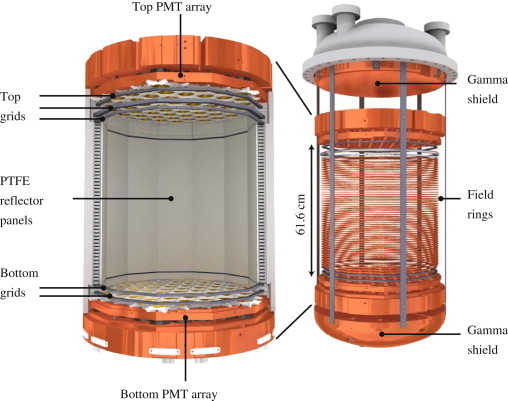
\includegraphics[width=\linewidth]{Figures/lux_internals.jpg}
\caption{}
\end{subfigure}%
\begin{subfigure}{0.5\linewidth}
\centering
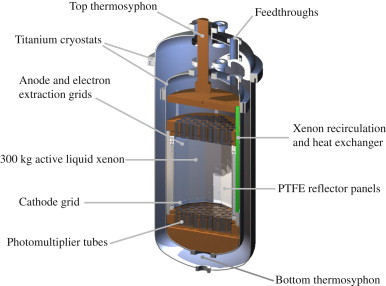
\includegraphics[width=\linewidth]{Figures/lux_layout.jpg}
\caption{}
\end{subfigure}
\caption{Layout of the LUX internals.\cite{lux2012}}
\label{fig:lux_layout} 
\end{figure}

The electric fields in LUX were set by five parallel-wire grids. There is a ``top'' and a ``bottom'' grid, which shielded the PMT arrays from seeing the full extent of the drift and extraction fields. The PMT's themselves are contained within two copper mounting blocks, with reflective Teflon covering the gaps between the PMT faces. The extraction field was set by the anode, which is about 1 cm above the liquid surface, and the gate grid, which is about 5 mm under the liquid surface. The drift field is set by the gate grid and the cathode, which are both submerged in the liquid, and are separated by 49 cm. The uniformity of the drift field is enforced by a set of 48 field rings which are separated by 1 cm distance and are connected to their adjacent rings by two 1 G$\Omega$ resistors. The top ring is connected to the gate by a 0.875 G$\Omega$ resistor pair, and the bottom ring is connected to the cathode by a 1.25 G$\Omega$ resistor pair. Charging of the Teflon walls, which resulted from a grid conditioning campaign, caused the drift field to become non-uniform after the first data-taking run. This will be described further in section \ref{sec:efield}.

The field rings are supported by a UHMW polyethylene structure. The interior side of this structure is covered by 12 reflective Teflon panels. This gives the active xenon region a 47cm diameter, dodecagonal shape. Also embedded in the polyethylene structure is a 2-phase heat exchanger and a weir. The heat exchanger allows for heat transfer between the inlet and outlet sides of the xenon circulation, and the pour-over weir maintains a precise liquid level.

The temperature of the xenon is cooled and maintained at about 170K by a pair of copper shields at the top and bottom of the inner cryostat, which also act to block gammas. The copper shields themselves are cooled by a thermosyphon system\cite{thermosyphon}. A thermosyphon transfers heat from a cold head to a liquid nitrogen-cooled condenser through a double-walled tube filled with nitrogen gas. The nitrogen gas condenses on the condenser and drips down the inner wall until it reaches the cold-head. It vaporizes on the cold head and the newly warmed gas travels up the tube between the inner and outer walls back to the condenser. The cooling power can be regulated by adjusting the nitrogen pressure within the tube.

A gas recirculation system allowed the xenon to be constantly purified, which was done using a SAES
MonoTorr heated-zirconium getter\cite{getter}. The xenon was circulated through this getter by a diaphragm pump at a rate of about 20-25 standard liters per minute (SLM). Of this flow, 15-20 SLM came from the output of the 2-phase heat exchanger, and another 5 SLM came from instrumentation purge lines. This recirculation system also provided access to an in-situ sampling system for purity analysis, a liquid nitrogen cooled recovery vessel, the long-term xenon storage cylinders, and the tritium\cite{lux_tritium} and krypton-83m\cite{lux_kr1} internal-source injection systems. These injection systems are designed to mix samples of radioactive gasses into the xenon, allowing calibrations to be performed where the events are uniformly distributed throughout the active region.

\subsection{Data Structure}
There are three levels of data storage files used by LUX. All of the PMT waveform data that passes some minimum threshold is digitized into .dat files. This minimum threshold is defined such that any signal equal or greater than a single photo-electron will be digitized. 

These .dat files are fed into a set of code referred to as the ``Event Builder'', which filters the PMT waveforms into collections called ``events''. For an event to be triggered, a more stringent threshold must be crossed. This threshold requires, in part, multiple PMT's to fire in coincidence. When an event is triggered, an ``event window'' is defined, which spans 1 millisecond  before and after the event trigger. Peaks in the PMT waveforms found within this event window are further sorted into a set of 10 ``pulses''. The events and pulses are then stored in .evt files.

The highest level file is the .rq file. These files are output by the data processing framework, which sorts the pulses into $S1$, $S2$, single extracted electron, single photo-electron, or other. The framework also calculates all of the quantities of interest, such as the x-y positions, efficiency corrections, drift time, pulse timing, etc..


\subsection{Electric Field Model}\label{sec:efield}
After the first WIMP-search run (Run03), and before the final WIMP-search run (Run04), LUX underwent a grid conditioning campaign modeled after a burn-in period of a proportional counter. After this campaign was completed, it was found that the drift field had become highly non-uniform. The altered field is best explained by charge build-up on the Teflon panels.
\begin{figure}[!h]
\centering
\begin{subfigure}{0.5\linewidth}
\centering
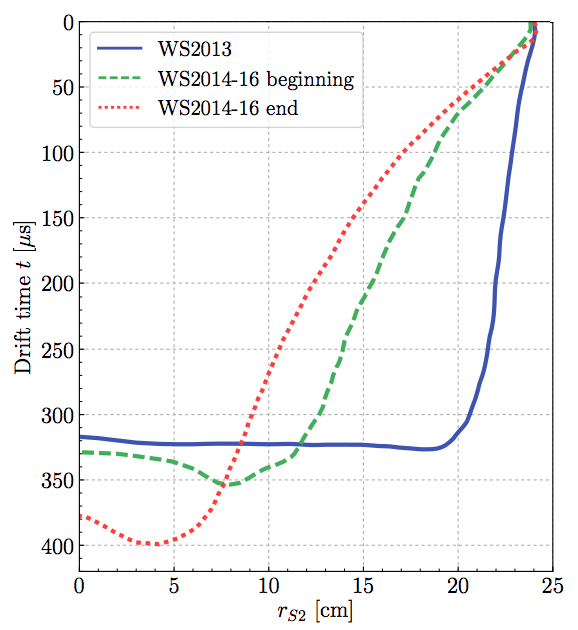
\includegraphics[width=\linewidth]{Figures/wall_radius.png}
\caption{}
\end{subfigure}%
\begin{subfigure}{0.5\linewidth}
\centering
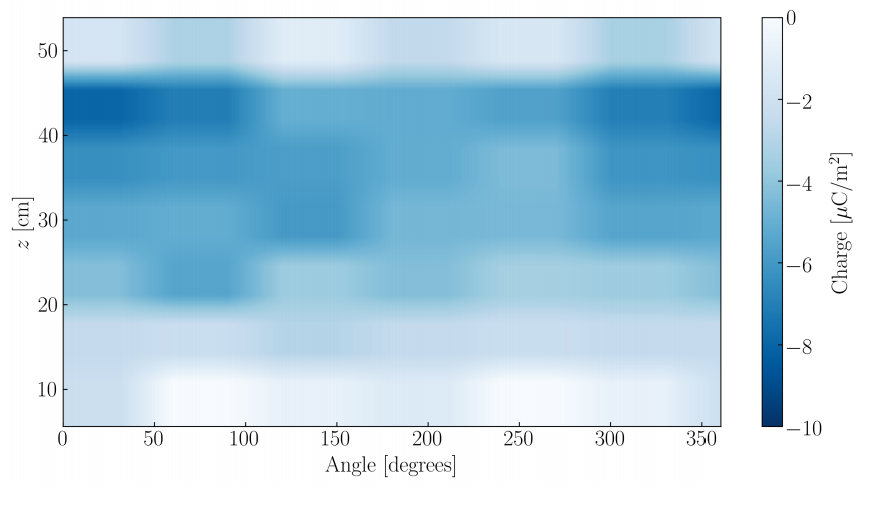
\includegraphics[width=\linewidth]{Figures/wall_charge.png}
\caption{}
\end{subfigure}
\caption{Here is shown the observed $S2$ x-y position of events at the wall of the detector (a), and an example of a best-fit charge distribution (b). The lines labeled WS2014-16 indicate data from the Run04 WIMP-search, and the WS2013 line shows the Run03 data. The reduction in wall radius at high drift times in the Run04 lines indicates that the drift field is highly non-uniform. The distribution of the wall-charge shown in (b) is for $^{83m}$Kr dataset from Kr data from 2014-10-06 and corresponds to the ``WS2014-16 beginning'' line. Figure taken from \cite{lux_efield}.}
\label{fig:lux_layout} 
\end{figure}

The uniformity of the drift field can be tested by analyzing the distribution of $^{83m}$Kr events after an injection. The $^{83m}$Kr quickly becomes uniformly mixed throughout the active region, so the observed positions of the events should be uniformly distributed in drift time, as well as the x-y position of the $S2$. After the grid conditioning, it was found that at longer drift times the x and y position of the $S2$ became compressed. The distortion of the distribution indicated that a $^{83m}$Kr event that occurred near the wall of the detector (about 23.5 cm radius) at 300 microseconds drift time would have an $S2$ position of about 13 cm radius. Since electrons trace the electric field, this indicates that the field lines were not vertical and parallel, and that therefore the electric field was not uniform.

A comprehensive study of the drift-field in LUX was performed and is detailed in \cite{lux_efield}. For this analysis, the wall was divided into 42 tiles. A test-charge was placed on each of these tiles, and the resulting electric field was calculated using a COMSOL model. These 42 electric fields, along with a 0-charge field, are combined using the superposition principle, creating a net field that is used to generate a simulated $^{83m}$Kr dataset. The best-fit charge distribution is found by adjusting the weights of this superposition and comparing the resulting $^{83m}$Kr simulation to data.
 
 \subsection{Efficiency Corrections}\label{sec:krypcal}
The efficiency at which photons and electrons are converted into $S1$ and $S2$ vary depending on position at which they were generated. For instance, consider an event with energy $E$, number of photons, $N_{\gamma}$, and number of electrons, $N_e$. The top PMT array has a lower collection efficiency than the bottom array, so if this event takes place near the top of the detector it would create a smaller $S1$ signal than if it was at the bottom. The $S2$ efficiency works in the opposite direction. Electrons generated near the bottom of the detector have to travel farther before they reach the liquid surface and therefore have a greater chance of being absorbed by a chemically active impurity. 

The average conversion factors from $N_{\gamma}$ and $N_e$ to $$S1$$ and $S2$ are referred to as $g1$ and $g2$:
\begin{equation}\label{eq:krypcal1}
\begin{split}
\langle S1 \rangle = N_{\gamma}g1\\
\langle S2 \rangle = N_e g2
\end{split}
\end{equation}
The variation in the efficiencies can therefore be thought of as a position dependence in these conversion factors ($g1=g1(xyz)$ and $g2=g2(xyz)$). We only have access to the ultimate $S1$ and $S2$ signals generated by an event, but the quantities we are interested in measuring are $N{_\gamma}$ and $N_e$. In order to extract these values, signal corrections are applied to $S1$ and $S2$ in order to remove the position dependence of $g1$ and $g2$. These corrections are defined:
\begin{equation}\label{eq:krypcal2}
\begin{split}
C_{S1}(xyz) \equiv \frac{g1(center)}{g1(xyz)}\\[1em]
C_{S2}(xyz)\equiv \frac{g2(top)}{g2(xyz)},
\end{split}
\end{equation}
where the center and top of the detector are indicated by $center$ and $top$. Then a single average value of each conversion factor is measured ($G1$ and $G2$) and used to calculate expected $N_{\gamma}$ and $N_e$ for an event with observed $S1$ and $S2$:
\begin{equation}
\begin{split}
\langle N_{\gamma} \rangle = \frac{S1_c}{G1}\\[1em]
\langle N_e \rangle = \frac{S2_c}{G2},
\end{split}
\end{equation}
where the subscript, $c$, represents an efficiency corrected value ($S1(2)_c=S1(2)\cdot C_{S1(2)}$).

While $g1$ and $g2$ vary with position, $N_{\gamma}$ and $N_e$ will depend on both the energy of the event, as well as the electric field. The non-uniform electric field described in the previous section means that an event with energy $E$, will produce a different $N_{\gamma}$ and $N_{e}$ depending on where it occurrs in the detector. This is problematic to the measurements of $C_{S1}(xyz)$ and $C_{S2}(xyz)$. Typically the signal corrections are measured by assuming that $N_{\gamma}$ and $N_{e}$ from a line source will be constant throughout the detector. In this case, the efficiency corrections can be simply measured using:
\begin{equation}\label{eq:krypcal3}
\begin{split}
\frac{\overline{S1}(center)}{\overline{S1}(xyz)}\approx \frac{N_{\gamma}(center)g1(center)}{N_{\gamma}(xyz)g1(xyz)}\\[1em]
\frac{\overline{S2}(top)}{\overline{S2}(xyz)}\approx \frac{N_{e}(top)g1(top)}{N_{e}(xyz)g1(xyz)},
\end{split}
\end{equation}
where $\overline{S1}(xyz)$ and $\overline{S2}(xyz)$ are the average values measured from events at a given position, and we have made the approximation that $\overline{S1}(xyz)=\langle S1(xyz) \rangle$ and $\overline{S2}(xyz)=\langle S2(xyz) \rangle$. When $N_{\gamma}$ and $N_e$ are constant in position, as would be true for a line source in a uniform electric field, the terms $\frac{N_{\gamma}(top)}{N_{\gamma}(xyz)}$ and $\frac{N_{e}(top)}{N_{e}(xyz)}$ would cancel, leaving us with the expressions for $C_{S1}(xyz)$ and $C_{S2}(xyz)$ shown in equation \ref{eq:krypcal2}. 

Since the field is not uniform in LUX Run04 and onward, a field-correction is applied to the $S1$ and $S2$ signals before the efficiency-corrections could be found:
\begin{equation}\label{eq:krypcal4}
\begin{split}
S1_F\equiv S1 \frac{\langle N_{\gamma}(center) \rangle}{\langle N_{\gamma}(xyz)\rangle}\\[1em]
S2_F\equiv S2 \frac{\langle N_{e}(center)\rangle}{\langle N_{e}(xyz)\rangle}
\end{split}
\end{equation}
Here $S1_F$ and $S2_F$ are the field-corrected signals. Equation \ref{eq:krypcal2} can then be written
\begin{equation}\label{eq:krypcal5}
\begin{split}
C_{S1}(xyz) \equiv \frac{g1(center)}{g1(xyz)}=\frac{\langle S1(center) \rangle / N_{\gamma}(center)}{\langle S1(xyz) \rangle / N_{\gamma}(xyz)}\cdot \frac{N_{\gamma}(center)}{N_{\gamma}(center)} &\approx \frac{\overline{S1_F}(center)}{\overline{S1_F}(xyz)}\\[1em]
C_{S2}(xyz) \equiv \frac{g2(center)}{g2(xyz)}=\frac{\langle S2(top) \rangle / N_{e}(top)}{\langle S2(xyz) \rangle / N_{e}(xyz)} \cdot \frac{N_{e}(top)}{N_{e}(top)} &\approx \frac{\overline{S2_F}(top)}{\overline{S2_F}(xyz)}
\end{split}
\end{equation}

In Run04, the position-dependent efficiency corrections for the LUX $S1$ and $S2$ signals are obtained from a combination of tritium and $^{83m}$Kr calibration data using a procedure referred to as KrypCal\cite{richard}. The KrypCal procedure begins with measuring  $C_{S2}$ using tritium. The field-dependence of $N_{e}$ are at a minimum at low-energy, so the use of tritium limits the systematic effects introduced by the estimation of $\frac{\langle N_{e}(center)\rangle}{\langle N_{e}(xyz)\rangle}$. This estimation is made using the existing NEST model, which will be introduced in the next section, and by making the approximation that the continuous tritium beta spectrum is actually a line source at 2.5 keV. To track $\overline{S2_F}$ as a function of position, the detector is binned in x, y, and z, and the tritium $S2_F$ spectrum in each bin is fit to a Landau function. The peak values of these Landau fits are taken to be $\overline{S2_F}$.

Tritium is only injected every 3 months or so, while the $^{83m}$Kr injections take place multiple times a week. For this reason, the ultimate measurements of $C_{S1}$ and $C_{S2}$ are made using krypton data. The field corrections for the krypton-83m events are derived using the preliminary tritium $S2$ corrections. Applying this preliminary efficiency correction to the $^{83m}$Kr $S2$ signals reveals the field dependence of $\langle N_{e}(xyz)\rangle$. Using the combined energy-model presented in section \ref{sec:combE}, the field dependence of $\langle N_{\gamma}(xyz)\rangle$ is derived from that of $\langle N_{e}(xyz)\rangle$. These field dependences give the field corrections for both the $^{83m}$Kr $S1$ and $S2$ signals. These field-corrections are propagated to each $^{83m}$Kr dataset, and the efficiency-corrections are calculated.

\section{Signals in Liquid Xenon and their Variations}
\subsection{The Combined Energy Model}\label{sec:combE}
When an energetic particle interacts with a target xenon atom it will create two measurable excitations, ions and excitons, with the rest of the energy being lost to heat. The expression for the energy of the interaction can then be written:
\begin{equation}\label{eq:combe1}
\begin{split}
E&=fW(N_*+N_i)\\
&=fW(1+\alpha)N_i,
\end{split}
\end{equation}
where $f$ is a loss factor to account for the energy that goes into heat, $N_*$ is the number of excitons generated in the event, and $N_i$ is the number of ions. The work function $W$ represents the average amount of energy it takes to produce a single ion or exciton. The quenching factor $f$ is constant for ER events, and so gets folded into the measurement of $W$. For NR events $f$ depends on the energy of the recoil and so cannot be hidden in the same way. In these cases, the typical approach is to take $W=W_{ER}$ and to express $f$ in terms of the Lindhard factor, $L$\cite{lindhard}:
\begin{equation}
\begin{split}
E_{ER}=W(N_*+N_i)\\[1em]
E_{NR}=\frac{W}{L}(N_*+N_i)
\end{split}
\end{equation}
For ER events, the work function has been measured to be $W=13.7 \ \pm0.2$ eV/quanta\cite{dahl}. We have also defined the exciton-ion ratio $\alpha \equiv N_{*}/N_{i}$, which has been measured to be about 0.2\cite{doke2002,attila} for ER events and is typically assumed to be constant. In this document we will take $\alpha$ to have a constant value of 0.18 for ER events. 

Excitons are short-lived xenon molecules, Xe$_2^*$, in which a single excited xenon atom is able to bond with a ground state atom, in either a singlet or triplet state. The singlet state has a lifetime of about 3.1 ns, whereas the triplet state lives for about 24 ns\cite{pulseshape}. Both the singlet and triplet states decay to 2Xe by emitting two 178nm photons which contribute to the primary scintillation light ($S1$). Since these photons are emitted by the diatomic Xe$_2^*$, they are not readily absorbed by monatomic xenon and so will travel through the detector unimpeded. 

Some of the exciton-ion pairs will recombine to form additional Xe$_2^*$ molecules, and therefore also more primary scintillation light. The recombination process happens with a time constant of less than 50 ns\cite{rectime}. Assuming a fraction $r$ of electron-ion pairs recombine, the total number of photons $N_{\gamma}$ and electrons $N_{e}$ produced in an event would be given by:
\begin{equation}\label{eq:combe2}
\begin{split}
N_{\gamma}&=N_*+rN_i\\
&=(\alpha+r)N_i\\
N_e&=(1-r)N_i
\end{split}
\end{equation}
The recombination fraction, $r$, will be randomly distributed where both the mean value, $P_R$, and standard deviation, $\sigma_R$, depend on the decay energy and electric field.

Averaging equation \ref{eq:krypcal1} and combining with equations \ref{eq:combe1} and \ref{eq:combe2} yields a relation between the energy of an ER event and the average values of the observables, $S1_c$ and $S2_c$ :
\begin{equation}\label{eq:combe3}
E_{ER}=W(\frac{\overline{S1_c}}{G1}+\frac{\overline{S2_c}}{G2})
\end{equation}
Dropping the averages on the right side gives the expression for reconstructed energy: 
\begin{equation}\label{eq:combe3}
E_{rec}=W(\frac{S1_c}{G1}+\frac{S2_c}{G2})
\end{equation}
Reconstructed energy is an observable quantity that fluctuates around the true energy of the event, so can therefore be thought of as a measure of the true energy.
\begin{figure}[!h]
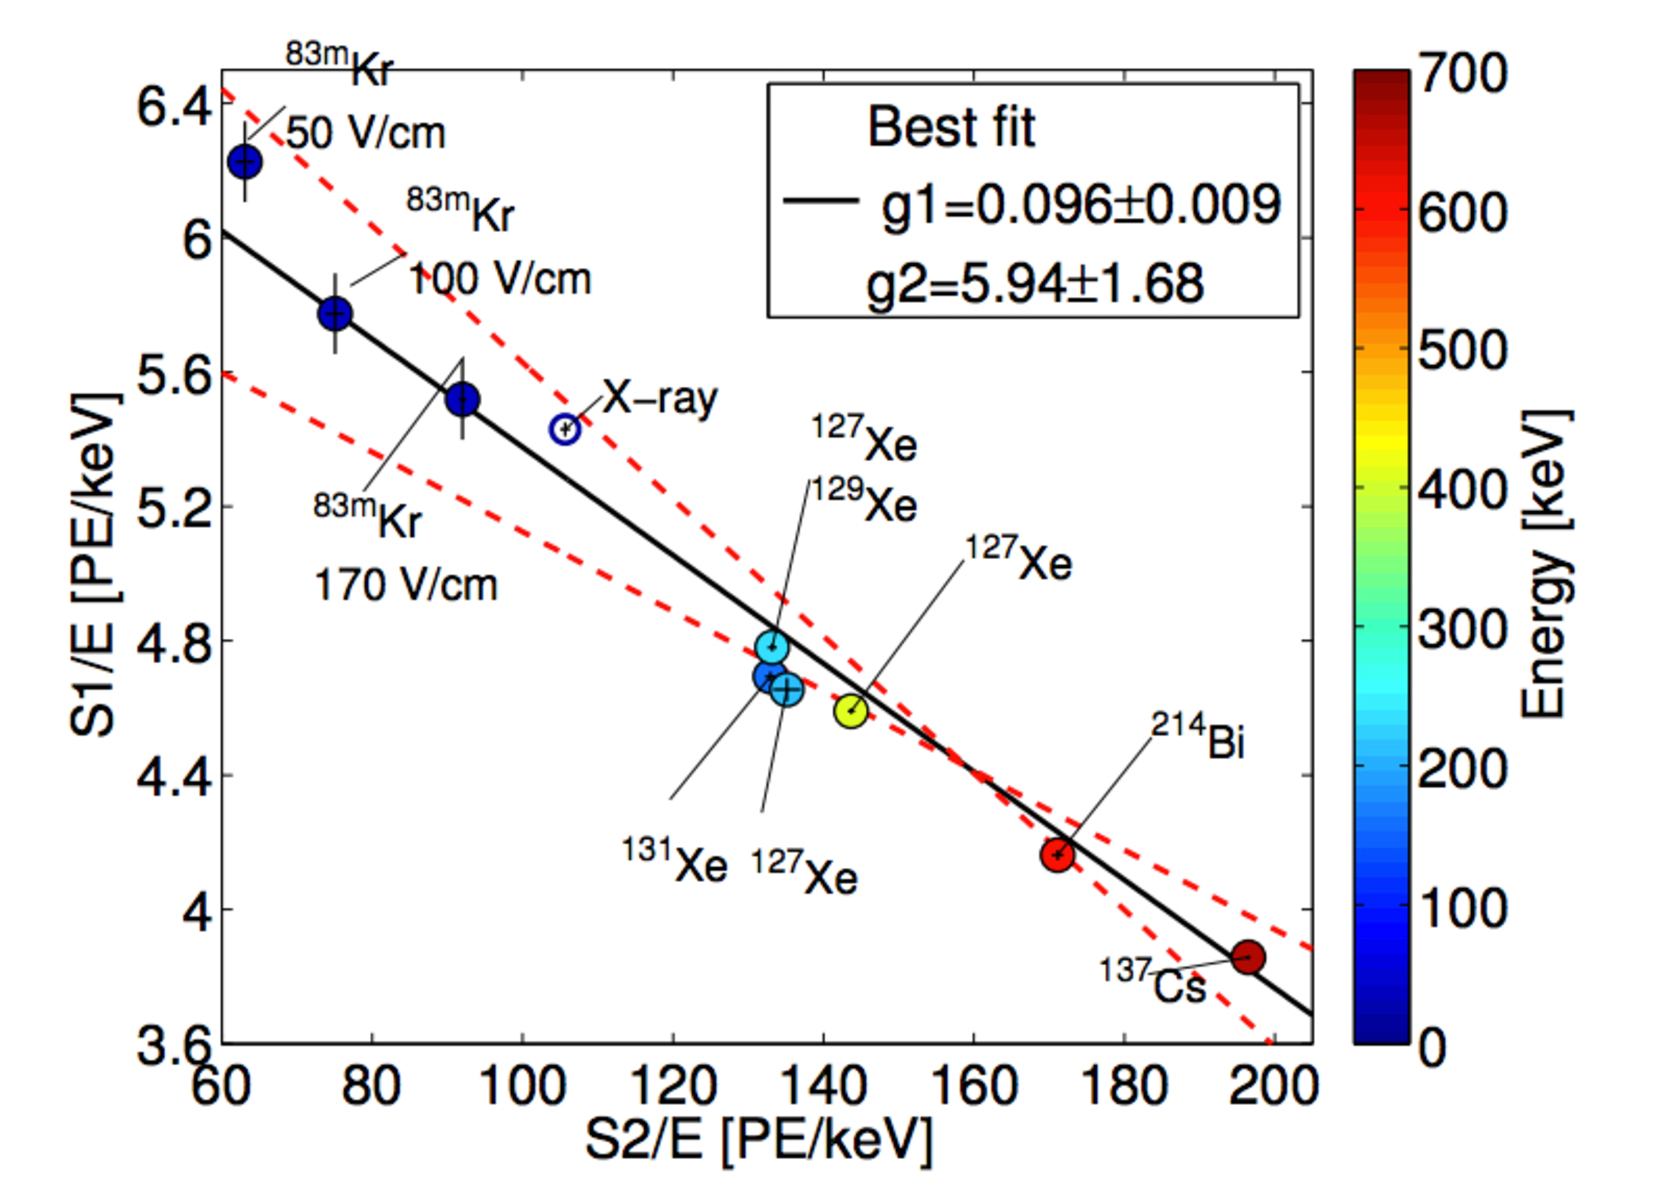
\includegraphics[width=\linewidth]{Figures/Doke_plot_run03.pdf}
\caption{Doke plot measured using various calibration lines in LUX Run03. Figure taken from \cite{attila}.}
\label{fig:lux_doke_plot} 
\end{figure}

Equation \ref{eq:combe3} also provides a useful tool in measuring the efficiency factors, $G1$ and $G2$. For an ER event with known energy $E$, we can write:
\begin{equation}
\left(\frac{W\overline{S1_c}}{E}\right)=-\frac{G1}{G2}\left(\frac{W\overline{S2_c}}{E}\right)+G1
\end{equation}
This equation has the form of a line where $y=\left(\frac{W\overline{S1_c}}{E}\right)$ and $x=\left(\frac{W\overline{S2_c}}{E}\right)$ are both in terms either measurable quantities or known constants. The efficiency factors, $G1$ and $G2$, can then be obtained by fitting a line through a set of (x,y) values measured at different energies and/or fields. This is referred to as the Doke plot method, and is the most common method for measuring $G1$ and $G2$\cite{doke2002}.

\begin{figure}[!h]
\centering
\begin{subfigure}{\linewidth}
\centering
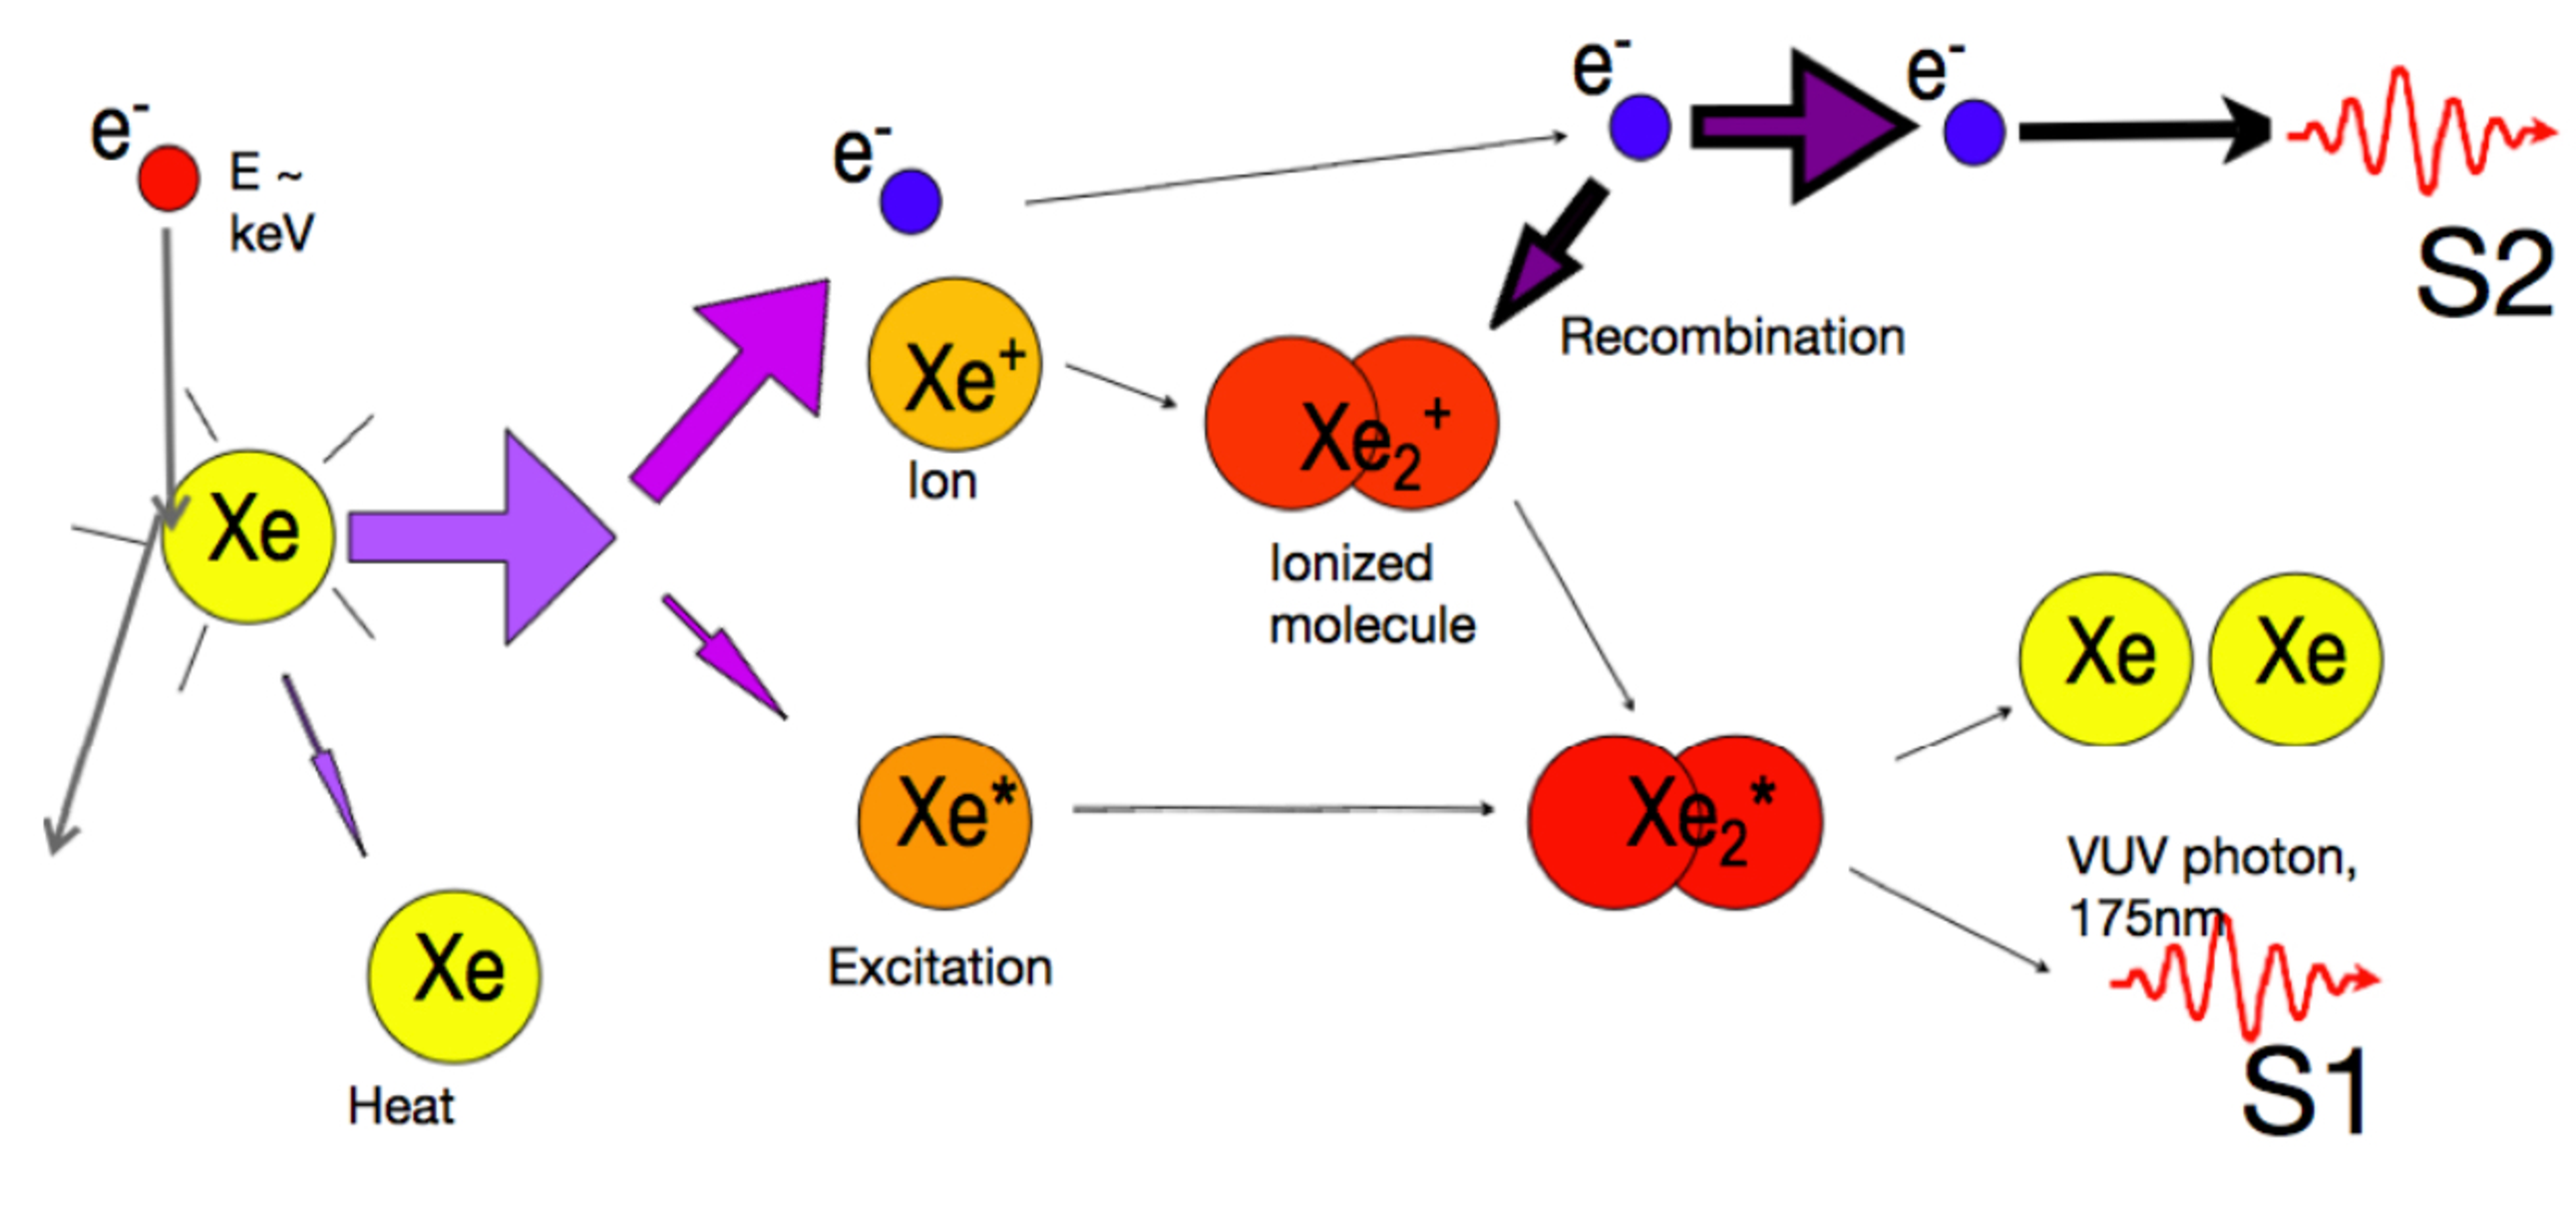
\includegraphics[width=\linewidth]{Figures/ER_diagram.pdf}
\caption{}
\end{subfigure}
\begin{subfigure}{\linewidth}
\centering
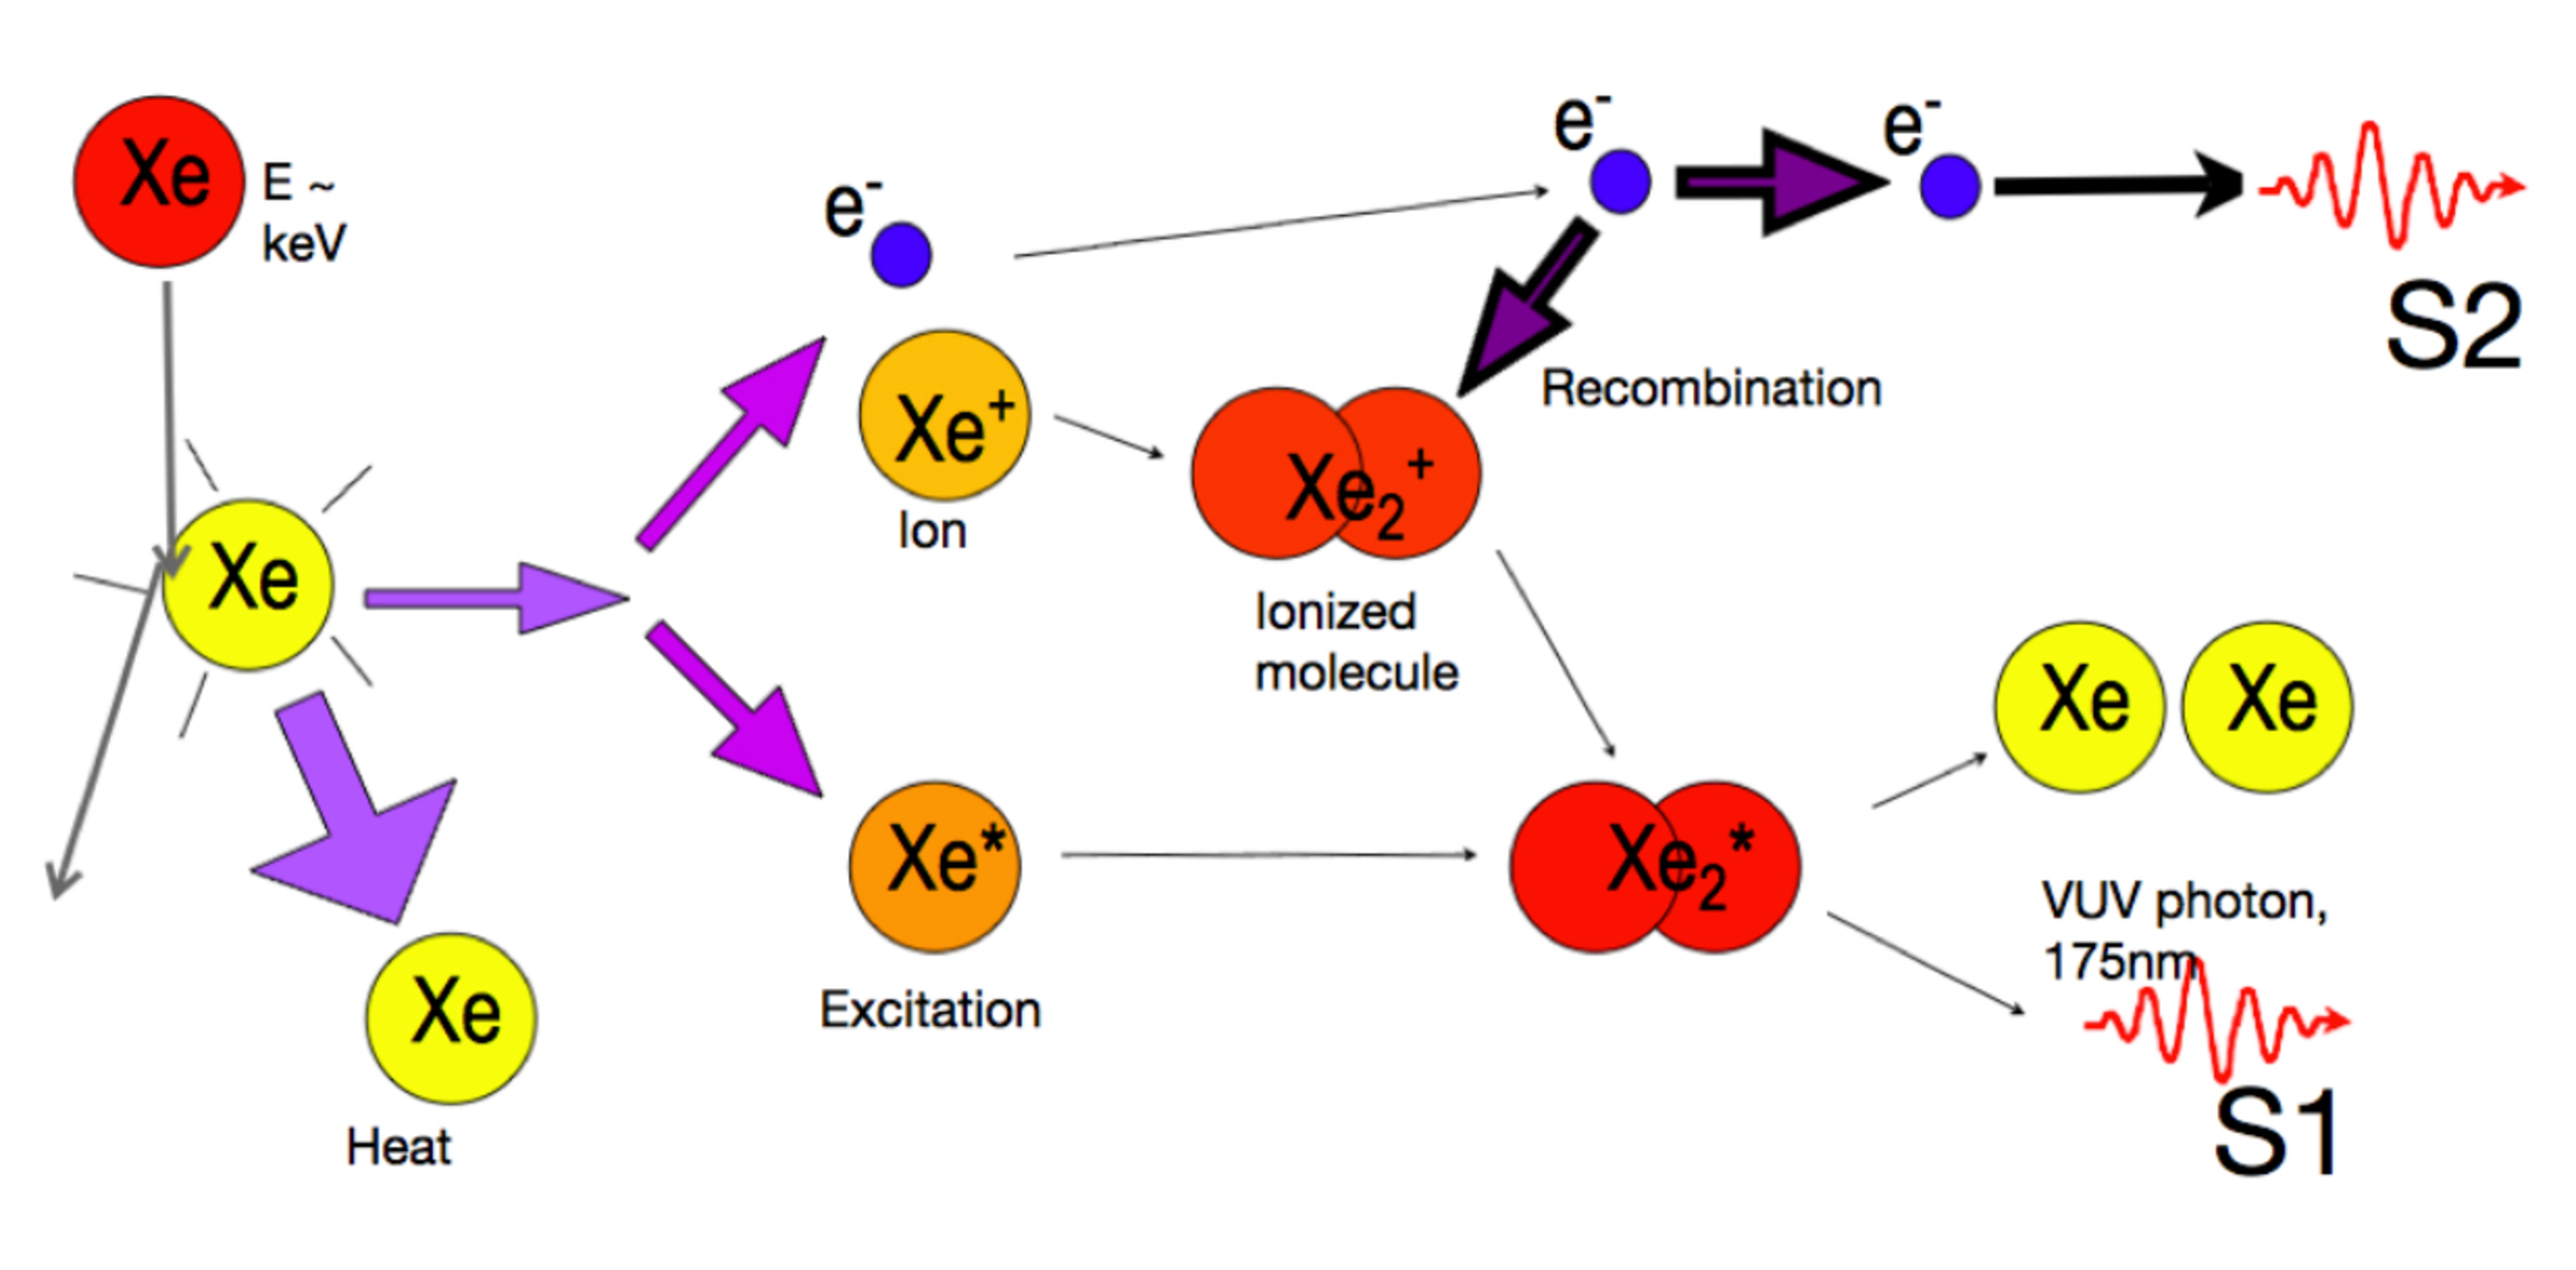
\includegraphics[width=\linewidth]{Figures/NR_diagram.pdf}
\caption{}
\end{subfigure}
\caption{Diagrams of an electronic recoil (a) and a nuclear recoil (b). These figures show how the deposited energy becomes partitioned between charge, light, and heat. In ER events, the amount of energy that goes into the heat channel is negligible. For NR events, however, a significant portion of the event energy is transferred to heat and is therefore not observed. Figures taken from \cite{attila}.}
\label{fig:lux_layout} 
\end{figure}



\clearpage

\subsection{Detector Resolution for Charge and Light Signals}\label{sec:detres}
On top of the fluctuations due to the recombination process, the $S1$ and $S2$ signals will also fluctuate due to detector variations. The $S1$ detector resolution, $\sigma_{\gamma,det}$ is composed of three parts: the binomial variance due to the finite light collection efficiency, $\epsilon_{\gamma}$:
\begin{equation}
\sigma_{S1,col}^2=N_{\gamma}G1(1-G1), 
\end{equation}
an additional variance due to a nonzero probability, $P_{DPE}$, that the PMT will experience double-photoemission\cite{DPE}:
\begin{equation}
\sigma_{S1,DPE}^2=G1\cdot N_{\gamma}P_{DPE}(1-P_{DPE}), 
\end{equation}
and the variance due to finite PMT resolution, $\sigma_{PMT}$:
\begin{equation}
\sigma_{S1,PMT}=N_{\gamma}G1\sigma_{PMT}^2
\end{equation}
The LUX signals were corrected for the double-photoemission effect, and so the $S1$ and $S2$ signals are measured in photons-detected (phd) rather than the typical photo-electrons (phe). For LUX post-Run04, we have $G1\approx 0.095$ phd per photon, $P_{DPE}\approx 0.2$, and $\sigma_{PMT}\approx 0.37$. Put together, this gives:
\begin{equation}
\begin{split}
\sigma_{S1,det}^2&=N_{\gamma}G1(1-G1+P_{DPE}(1-P_{DPE})+\sigma_{PMT}^2)\\
&\approx 0.11 \cdot N_{\gamma} \ \ (\text{phd}^2)
\end{split}
\end{equation}

The $S2$ signals are a bit more complicated because there are more steps between the initial generation of electrons, and the final detection of the secondary scintillation light. First, a fraction ($1-\kappa$) of the electrons will be lost as they travel from the interaction site to the liquid surface, and then another fraction will be lost due to finite extraction efficiency ($\epsilon_e$). We model these two effects with a single binomial distribution with probability equal to $\kappa\epsilon_e$. In LUX post-Run04, $\overline{\kappa} \approx 0.95$ and $\epsilon_e \approx 0.7$, so the total variance in the number of extracted electrons is:
\begin{equation}
\sigma_{ee}^2=N_e\cdot \kappa\epsilon_e(1-\kappa\epsilon_e)\approx 0.22 \cdot N_e \ (\text{phd}^2)
\end{equation}

Once the electrons are extracted, there will be added variance in the measured $S2$ from fluctuations in the number of photons generated by the electron cascade, as well as from photon detection fluctuations analogous to those for the $S1$ signal. These fluctuations can be folded together into the width of the single electron (SE) spectrum, which is easily measured. Measuring the SE spectrum is also useful because it allows the extraction efficiency to be separated from the total $G2$ value:
\begin{equation}
\epsilon_e=\frac{G2}{\mu_{SE}}
\end{equation}
In LUX post-Run04, the single electron mean ($\mu_{SE}$) and width ($\sigma_{SE}$) were measured to be 24.5 and 5.3 phd, respectively. The total variance in $S2_c$ due to detector fluctuations will then be given by:
\begin{equation} 
\begin{split}
\sigma_{S2,det}^2&=N_e\cdot \kappa\epsilon_e(1-\kappa\epsilon_e)\mu_{SE}^2+N_e\cdot\kappa\epsilon_e\sigma_{SE}^2\\
&\approx 152 \cdot N_e \ (\text{phd}^2)
\end{split}
\end{equation}
 
The resolution of the reconstructed energy is given by:
\begin{equation}
\begin{split}
\sigma_{rec}^2&=W^2\left(\frac{\sigma_{S1,det}^2}{G1^2}+\frac{\sigma_{S2,det}^2}{G2^2}\right)\\[1em]
&=W^2\left((3.6)^2\cdot N_{\gamma}+(0.72)^2\cdot N_e \right)
\end{split}
\end{equation}
The energy resolution is therefore dominated by the $S1_c$ fluctuations. Assuming that $N_{\gamma}\approx N_e$, the energy resolution can be rewritten:
\begin{equation}
\sigma_{rec}^2\approx (0.3)^2\cdot E_{rec}
\end{equation}


\subsection{LibNEST: The Model Applied to LUX}\label{sec:libnest}
The Noble Element Simulation Technique (NEST) attempts to consolidate the various world measurements of energy deposition properties in liquid xenon into a single set of predictions\cite{nest1,nest2,lenardo}. The average charge and light signals measured experimentally are often reported using quantities referred to as light and charge yields:
\begin{equation}
\begin{split}
LY=\frac{\langle N_{\gamma}\rangle}{E}\\[1em]
QY=\frac{\langle N_e\rangle}{E}
\end{split}
\end{equation}
The expected number of photons and electrons for an event with energy $E$ can be calculated using the recombination model described in section \ref{sec:combE}:
\begin{equation}
\begin{split}
\langle N_{\gamma} \rangle=N_q\frac{\alpha +P_R}{1+\alpha}\\[1em]
\langle N_{e} \rangle=N_q\frac{1-P_R}{1+\alpha},
\end{split}
\end{equation}
where $\alpha=0.18$ is again the ion to exciton ratio, and $P_R$ is the expected recombination fraction for the event and is determined by the type of event, energy of the event, and applied drift field. The total number of quanta, $N_q$, is given by:
\begin{equation}
N_q=\frac{E}{W}=N_{i}+N_{*}=N_{\gamma}+N_{e}
\end{equation}
The equations for $LY$ and $QY$ can then be rewritten in terms of the recombination probability and the exciton-ion ratio, $\alpha$:
\begin{equation}
\begin{split}
LY=\frac{1}{W}\frac{\alpha +P_R}{1+\alpha}\\[1em]
QY=\frac{1}{W}\frac{1-P_R}{1+\alpha}
\end{split}
\end{equation}

A traditional model of recombination probability is inspired by Birk's Law is\cite{nest1}:
\begin{equation}\label{eq:birk}
P_R=\frac{A\frac{dE}{dx}}{1+B\frac{dE}{dx}}+C , \ B=A/(1-C)
\end{equation}
At energies less than about 1 MeV, the quantity $\frac{dE}{dx}$ tends to increase with decreasing energy. As $E$ becomes large (~1 MeV), the event tracks become long and the ion density more diffuse, leading to a smaller chance that an electron will encounter an ion and recombine. As $E$ goes to zero, equation \ref{eq:birk} predicts that $P_R$ should approach unity. This would correspond $LY=1/W$ and $QY=0$. It has been observed, however, that for energies below about 20 keV, $LY$ begins to decrease, and $QY$ increases. 

The current version of NEST relies on a model of recombination probability known as the ``Thomas-Imel Box'' model\cite{nest1,nest3,tib1,tib2}:
\begin{equation}\label{eq:tib}
P_R=1-\frac{\text{ln}(1+N_i\xi)}{N_i \xi} \text{,  where  } \xi \equiv \frac{\alpha'}{4a^2u_e\mathcal{E}}
\end{equation}
Here, $N_i$ is again the initial number of ions generated by an event, $\alpha'$ characterizes the dielectric properties of liquid xenon, and the mean velocity of electrons is given by the electron mobility, $u_e$, times the electric field, $\mathcal{E}$\cite{dahl}. The Thomas-Imel model assumes that the electrons and ions are initially uniformly distributed throughout a box with side length of $a$. At zero electric field, $a$ can be thought of as the thermalization distance in liquid xenon, or about 4.6 microns\cite{nest1}. This means that the model will work most naturally for low energy events, which have very short path lengths. Equation \ref{eq:tib} has no dependence on $\frac{dE}{dx}$, and instead only depends on $N_i$. As the event energy decreases, there are increasingly fewer ions contained in the box and so an electron becomes less likely encounter an ion and recombine as the energy decreases. Therefore, in contrast to the Birk model, the Thomas-Imel model reproduces the observed trend in $P_R$ as energy goes to 0. 

Dahl was the first to successfully apply a modified version of the Thomas-Imel model to event energies for which the path length exceeded the box size, $a$. To do this, he simulated particle tracks, accounting for the initial location of each ion created. Each ion was smeared into a box with side $a$, centered on its initial location, thus creating a set of mini Thomas-Imel boxes. In this way, Dahl created a new model that approaches the original Thomas-Imel version at low-energies and a more traditional columnar model in the high energy limit. Dahl calculated a best-fit $a$ parameter for a set of electric fields ranging from 60 to 4060 V/cm. He found the the box length was approximately proportional to $\mathcal{E}^{-1/2}$, with $\alpha \approx 2$ microns at 60 V/cm and $\alpha \approx 0.2$ microns at 4060 V/cm. He used this scaling to argue that the length scale of the recombination process is likely dominated by electrostatic effects, since the radius at which the electric field of an ion becomes greater than the drift field also has a $\mathcal{E}^{-1/2}$ dependence\cite{dahl}.

Currently, NEST uses equation \ref{eq:tib} as a functional form for a semi-empirical model of the recombination probability. In order to capture the effects due to path length and box size, the $\xi$ parameter is fit to a series of power-laws in electric field and energy, and therefore much of the physical meaning behind it is obscured. For ER energies less than 18.6 keV, the NEST model is tuned to the LUX Run03 tritium data\cite{lux_tritium}. Above 122 keV, the model tuned to data such as xenon activation lines and $^{57}Co$. Measurements between these values have historically been sparse, so the light and charge yields are interpolated in this region. The $^{14}$C measurements that will be presented in section \ref{sec:finalresults} will provide a powerful addition to the model because they probe this historically unknown region.

\begin{figure}[!h]
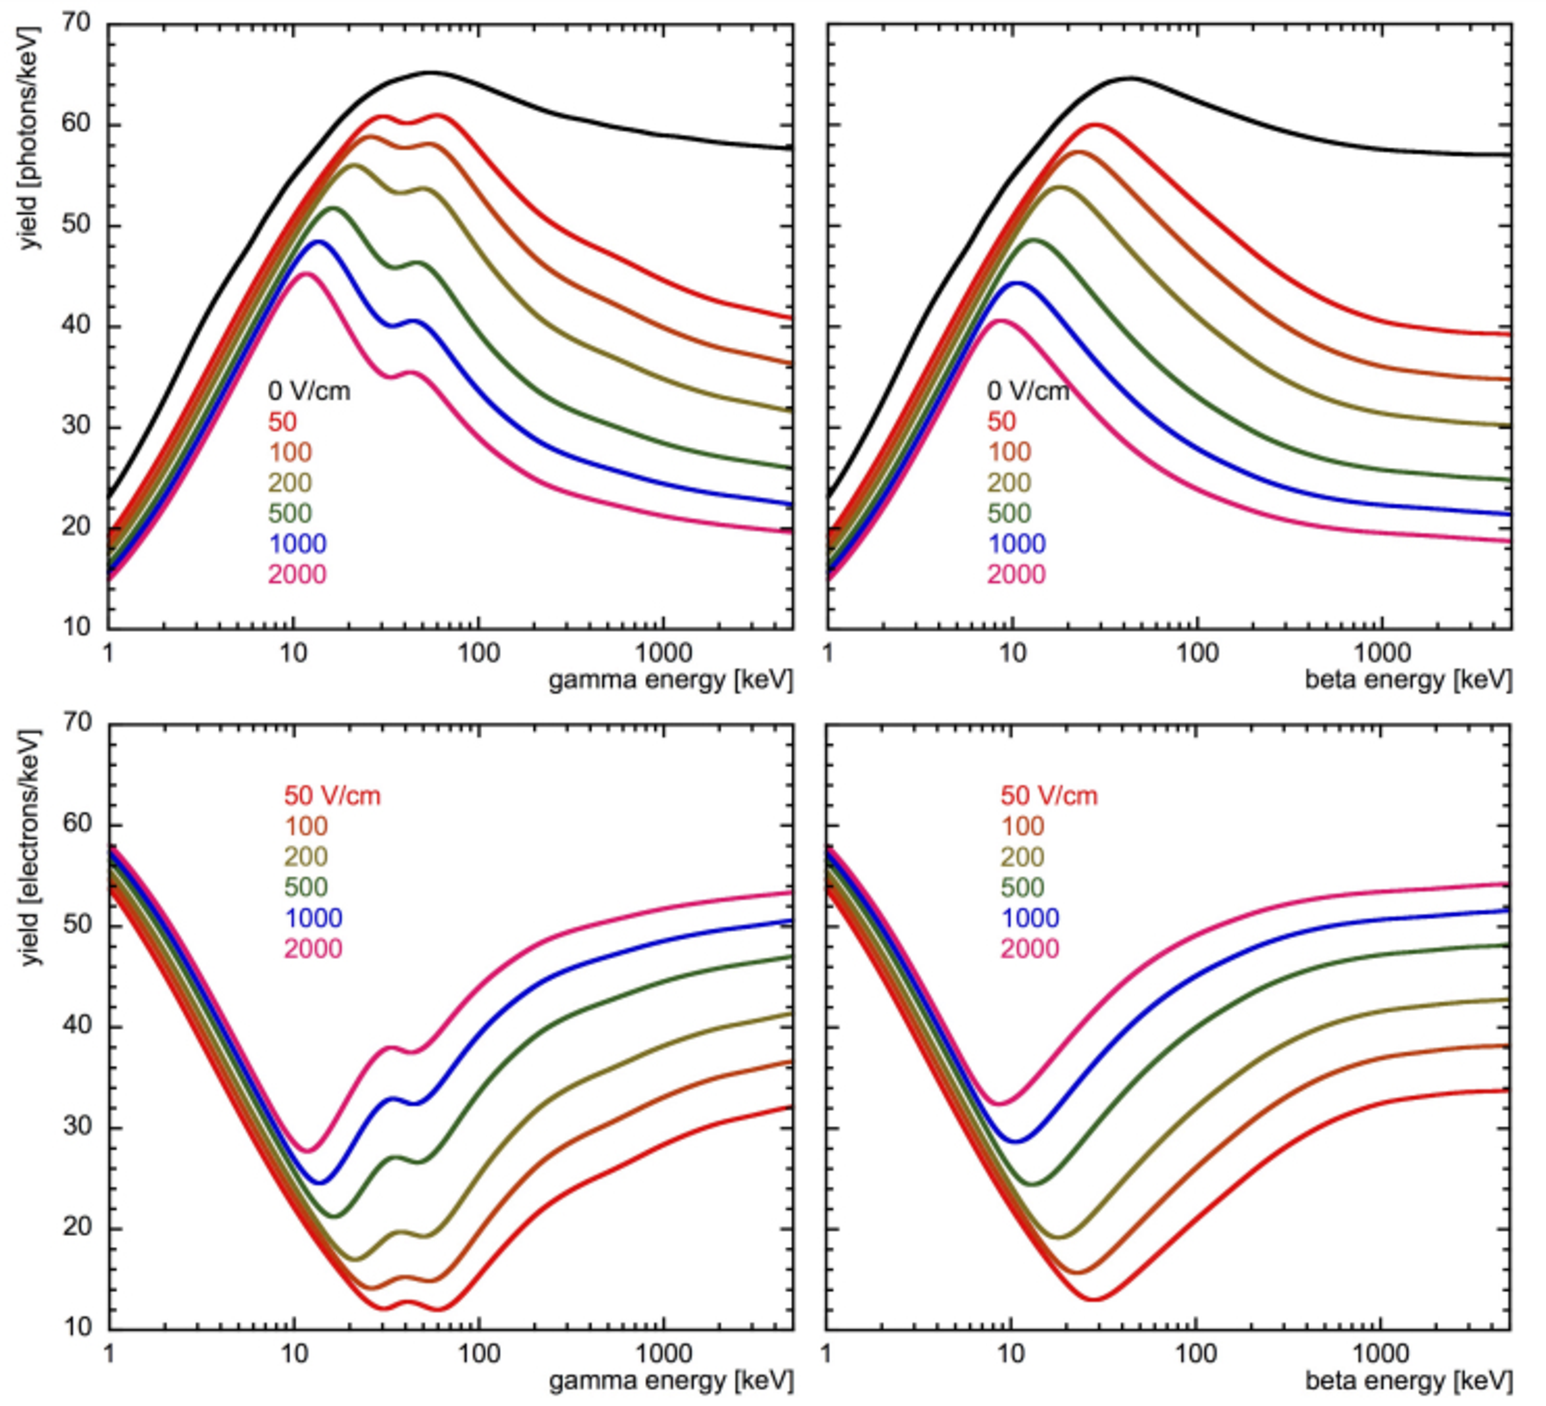
\includegraphics[width=\linewidth]{Figures/nest_yields0p98.pdf}
\caption{NEST v0.98 yield predictions for gamma (left) and beta/Compton (right) events. The bump in the gamma yields at 35 keV is due to photo-absorption at the K-edge x-ray site. Figure taken from \cite{nest2}.}
\label{fig:nest_yields0p98} 
\end{figure}


There are also considerations that must be made for whether the event is a beta of Compton scatter, or whether it is the photo-absorption of a gamma. The xenon K-edge x-ray will cause a resonance for gammas at 35 keV which is expected to increase the light yield in that region. The yield predictions from NEST v0.98 are shown in figure \ref{fig:nest_yields0p98}.

The recombination fluctuations are known to be greater than what would be expected for a binomial process. They have, in fact, been measured to grow approximately proportional to $N_i$\cite{attila}. NEST, therefore, models the recombination fluctuations using a Poissonian distribution, modified by a Fano-like factor, $F_RN_i$\cite{Evanyields}:
\begin{equation}
\sigma_R^2=(F_RN_i)\cdot (P_RN_i)
\end{equation}
\begin{table}[h!]
\centering
    \begin{tabular}{ c | c | c  }
    \hline
    parameter & description & value \\
    \hline \hline
    $G1^{\dagger}$ & average total light collection efficiency & 0.0931\\
    \hline
    $G2^{\dagger}$ & average total charge collection & 18.58\\
    \hline
    $\epsilon_e^{\dagger}$ & electron extraction efficiency ($G2$/$\mu_{SE}$) & 0.758\\
    \hline
    $\mu_{SE}$ & single electron mean & 24.5\\
    \hline
    $\sigma_{SE}$ & single electron width & 5.3\\
    \hline
    $\sigma_{PMT}$ & average resolution of PMTS & 0.37\\
    \hline
    $\kappa$ & probability of electron reaching liquid surface & sampled from $\frac{1}{C_{S2}}$\\
    \hline
    $F_R$ & Fano-factor for recombination fluctuations & 0.009975\\
    \hline
    \end{tabular}
    \caption{Values used in the libNEST model to simulate KrypCal corrected LUXdata in post-Run04 LUX data. The $\dagger$ superscript indicates values that will change when new efficiency corrections are introduced in section \ref{sec:corrections}.}
    \label{tab:libnestparms}
\end{table}


The libNEST code is a package developed for use with the LUX detector. It is designed to generate simulated LUX $S1$ and $S2$ signals given an input energy. It models the field and energy dependence of $N_{\gamma}$ and $N_e$ using the recombination model laid out in section \ref{sec:combE} and the NEST prediction of $P_R$ and $\sigma_R$. It then applies detector resolutions as described in section \ref{sec:detres} in order to generate the simulated $S1$ and $S2$ signals. The values of the parameters input into libNEST are shown in table \ref{tab:libnestparms}. This package will be used in chapters \ref{chap:4} and \ref{chap:5} of this document to model the effects of our new light and charge yield measurements on the $S1$ and $S2$ spectra for the ER calibrations conducted in LUX after the Run04 WIMP search.



